\section{Morphologischer Kasten}

\begin{figure}[H]
\centering
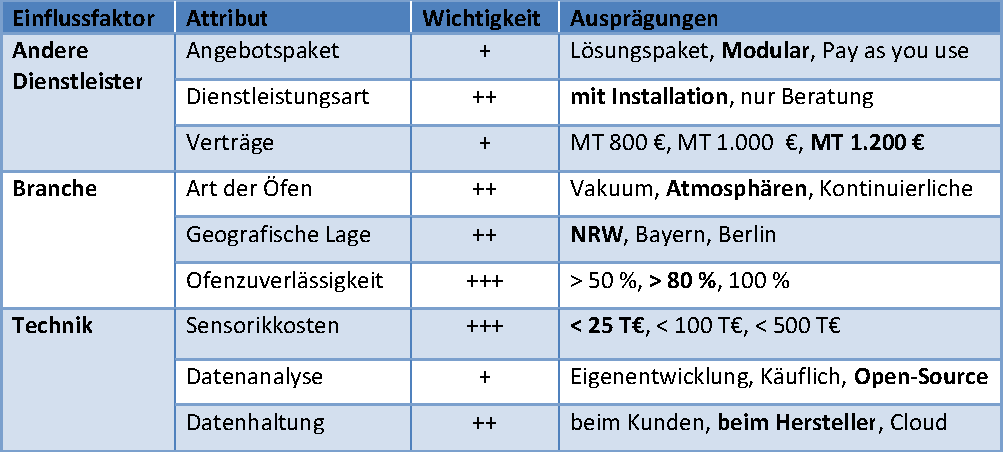
\includegraphics[width=0.9\linewidth]{Bilder/MorphologischerKasten}
\caption{Unser morphologischer Kasten}
\label{fig:MorphologischerKasten}
\end{figure}

Wir möchten als IT-Dienstleister im Bereich Predictive Maintenance für Hersteller von Atmosphärenöfen arbeiten. Dabei konzentrieren wir uns auf Hersteller im Raum NRW (z.B. der IVA in Dortmund), deren Öfen eine Zuverlässigkeit von mehr als 80 \% aufweisen. Für die Messung der Daten verwenden wir Sensorik deren Kosten unterhalb von 25.000 € liegen. Zur Analyse werden die Daten beim Ofenhersteller gespeichert und mit Hilfe von Open-Source-Lösungen ausgewertet. Unsere Angebotspakete sind modular aufgebaut, so dass aus unserem Dienstleistungsportfolio unterschiedliche Ausbaustufen in Anspruch genommen werden können. Neben der reinen Beratungsleistung bieten wir zusätzlich auch die Möglichkeit diese zu installieren. Für unsere Dienstleistung berechnen wir einen Tagessatz von 1.2000 €.
